\section{Results of the Runtime Verified AV System}

This research provides a solution for two aspects of \acf{AV} systems: predicting accurately with perturbations to the system's inputs and safely dealing with misclassifications by the system.
The issue of input perturbations was addressed using a \acf{MNN} of different convolutional \acfp{SNN}, each \ac{SNN} working in tandem to predict more accurately.
Misclassification by the system's controller was addressed by implementing sensor fusion between cameras and \ac{LiDAR}.
This was done using a run-time verifier that verified a safety automaton.
The benchmark was written in Esterel and C and run on Ubuntu 16.04, using an 4 core Intel i7-6700HQ processor at 2.6GHz and 4GB of RAM.

A graph was generated to show the affect of adversarial input perturbation, first presented as Figure~\ref{fig:sign-graph-acc} in Chapter 2.
It shows that the input perturbations decreased the accuracy of the classifiers by as much as 50\%.
However, the aim of this approach is not only to increase the classification accuracy of the \acp{MNN} but rather catch misclassifications made by the \acp{MNN}, i.e. verify that the classifications made by the \acp{MNN} are valid.
As such the results displayed do not show an increase in accuracy, but rather that the verifier is fully capable of catching misclassifications made by the \acp{MNN}.

To test the \ac{MNN}'s ability to deal with perturbations and misclassifications, the input images (taken from the \ac{VOC} 2012~\cite{pascal-voc-2012} and \ac{GTSRB}~\cite{Stallkamp2012-gtsrb} datasets) were perturbed by randomly replacing approximately 7\% of the image pixels with randomly coloured pixels.
The system was then run for over 10,000 ticks.
Each tick the classifier was presented an image to classify. 
The results of the overall classification was noted: did the \ac{MNN} controller make a misclassification and if so, was it caught by the run-time verifier.

\subsection{Results of the \ac{MNN} ensembles}
To test the efficacy of \ac{MNN} ensembles, three \acp{SNN} were trained on the data set.
These \acp{ANN} were then tested, individually, on both the original images and the same perturbed images and the results were noted in Table~\ref{tbl:sign-enemble}.
The overall average accuracy of three \acp{SNN} was also noted.
An ensemble made up of the three \acp{SNN} was then run on the exact same images and its classification accuracy noted.

\begin{table}[h]
	\centering
	\caption{Table showing the results of the \ac{MNN} ensemble}
	\label{tbl:sign-enemble}
	\begin{tabular}{|l||l|}
		\hline
		\ac{ANN} & Classification accuracy (\%) \\ \hline
		\multicolumn{2}{|l|}{Original Inputs} \\ \hline
		\ac{SNN} 1 & 84.24 \\ 
		\ac{SNN} 2 & 92.05 \\ 
		\ac{SNN} 3 & 89.62 \\ 
		\ac{SNN} Average & 88.64 \\
		\ac{MNN} Ensemble & 91.17 \\ 
		\hline
		\multicolumn{2}{|l|}{Perturbed Inputs} \\ \hline
		\ac{SNN} 1 & 56.52 \\ 
		\ac{SNN} 2 & 63.16 \\ 
		\ac{SNN} 3 & 62.85 \\ 
		\ac{SNN} Average & 60.84 \\
		\ac{MNN} Ensemble & 62.91 \\ 
		\hline
	\end{tabular}%
\end{table}

Table~\ref{tbl:sign-enemble} shows the impact of \ac{MNN} ensembles on the classification accuracy of images.
Without being in an ensemble, the overall classification accuracy of the \acp{ANN} was 88.64\% for the original images and 60.84\% for the perturbed images.
However, this average was increased to 91.17\% and 62.92\% for the original and perturbed images respectively.
Additionally, the ensemble performed significantly better than the ``worst'' \ac{SNN}.

While the \ac{MNN} ensemble did not perform better than the ``best'' \ac{SNN}, it did not perform significantly worse either.
This does not mean that the ensembles are useless.
When an \ac{ANN} is trained, it is not know before deployment whether that \ac{ANN} is a ``worst'' or a ``best''.
And while the ensemble does not increase the effectiveness of a ``best'' \ac{ANN}, it significantly increases the accuracy of a ``worst'' \ac{ANN}.
When ensuring timing and, in this case, functional safety of a system, the worst case must always be considered, and these ensembles will turn a worst case \ac{ANN} into a best case \ac{ANN}.

\subsection{Results of a Darknet~\cite{darknet13} implemented \ac{AV} system}
\begin{table}[h]
	\centering
	\caption{Table showing the results of the \ac{AV} prediction \ac{MNN}}
	\label{tbl:sign-resultsfull}
	\resizebox{\textwidth}{!}{%
		\begin{tabular}{|p{0.2\linewidth}||p{0.2\linewidth}|p{0.2\linewidth}|p{0.2\linewidth}|}
			\hline
			Epochs trained & No. of misclassifications (/100) & No. of caught misclassifications (/100) & \% of total misclassifications caught \\ \hline
			\multicolumn{4}{|l|}{Original Inputs} \\ \hline
			0 & 95.16 & 95.16 & 100 \\ 
			10 & 95.16 & 95.16 & 100 \\
			100 & 82.67 & 61.09 & 73.90 \\
			1000 & 29.36 & 21.39 & 72.85 \\
			10000 & 12.38 & 8.55 & 69.06 \\ 
			100000 & 11.98 & 7.79 & 65.03 \\
			6000 (best) & 10.59 & 7.32 & 69.12 \\ \hline
			\multicolumn{4}{|l|}{Perturbed Inputs} \\ \hline
			0 & 95.16 & 95.16 & 100 \\
			10 & 95.16 & 95.16 & 100 \\ 
			100 & 93.63 & 71.89 & 76.78 \\
			1000 & 76.69 & 63.71 & 83.07 \\
			10000 & 57.89 & 45.89 & 79.27 \\ 
			100000 & 58.03 & 45.72 & 78.79 \\
			7000 (best) & 60.42 & 49.13 & 81.31 \\ \hline
		\end{tabular}%
	}
\end{table}

The \ac{MNN} used in this system were trained for 10,000 epochs using the Darknet library~\cite{darknet13}.
Table~\ref{tbl:sign-resultsfull} shows the results of the Darknet generated classifier.
The first column shows the total number of misclassifications made, normalized to 100.
The second column shows the total number of misclassifications caught by the verifier, also normalized to 100.
The final column shows the relative percentage of the total misclassifications caught by the verifier.

Using the original inputs the verifier caught more than 65\% of the total misclassifications.
More than half of all the misclassifications made were detected by the verifier, and the safety of the system turned over to the driver.
This same table shows that when the inputs are perturbed, the verifier picked up more misclassifications than with the original images, catching more than 76\% of all misclassifications.
These results are summarised in Figure~\ref{fig:sign-graphboth}.

\begin{figure}[H]
	\centering
	\scalebox{0.9}{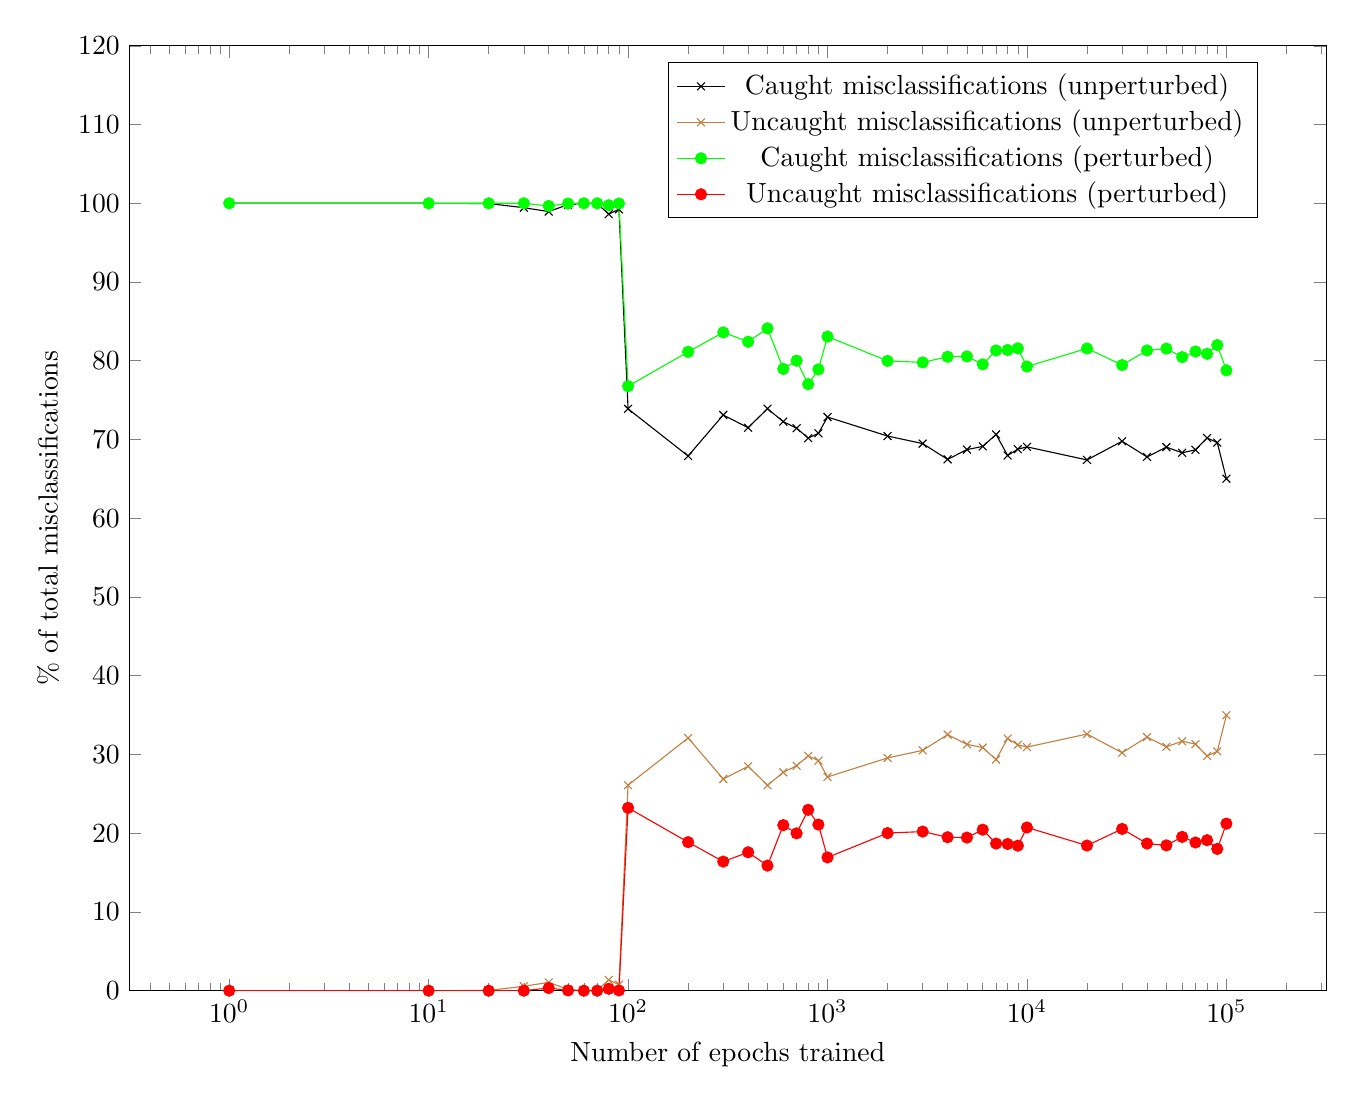
\begin{tikzpicture}
\begin{semilogxaxis}[
xlabel={Number of epochs trained},
ylabel={\% of total misclassifications},
x=1.1cm, y=1.0mm, 
ymin=0, ymax=120,
legend style={at={(0.45,0.9)},anchor=west}]

\addplot[color=black,mark=x] coordinates {
	(1, 100.000000)
	(10, 100.000000)
	(20, 99.968513)
	(30, 99.438622)
	(40, 98.948822)
	(50, 99.831619)
	(60, 100.000000)
	(70, 99.946243)
	(80, 98.629845)
	(90, 99.235352)
	(100, 73.896217)
	(200, 67.904327)
	(300, 73.114166)
	(400, 71.500191)
	(500, 73.917786)
	(600, 72.264412)
	(700, 71.438644)
	(800, 70.175438)
	(900, 70.787399)
	(1000, 72.854225)
	(2000, 70.439842)
	(3000, 69.480080)
	(4000, 67.477409)
	(5000, 68.717560)
	(6000, 69.121811)
	(7000, 70.645164)
	(8000, 67.972473)
	(9000, 68.772896)
	(10000, 69.063011)
	(20000, 67.405907)
	(30000, 69.780220)
	(40000, 67.787842)
	(50000, 69.032257)
	(60000, 68.315018)
	(70000, 68.693977)
	(80000, 70.194382)
	(90000, 69.604439)
	(100000, 65.025040)
};

\addplot[color=brown,mark=x] coordinates {	
	(1, 0.000000)
	(10, 0.000000)
	(20, 0.031486)
	(30, 0.561380)
	(40, 1.051184)
	(50, 0.168381)
	(60, 0.000000)
	(70, 0.053759)
	(80, 1.370155)
	(90, 0.764649)
	(100, 26.103786)
	(200, 32.095673)
	(300, 26.885832)
	(400, 28.499805)
	(500, 26.082212)
	(600, 27.735594)
	(700, 28.561354)
	(800, 29.824560)
	(900, 29.212601)
	(1000, 27.145777)
	(2000, 29.560154)
	(3000, 30.519920)
	(4000, 32.522587)
	(5000, 31.282434)
	(6000, 30.878185)
	(7000, 29.354836)
	(8000, 32.027523)
	(9000, 31.227106)
	(10000, 30.936995)
	(20000, 32.594090)
	(30000, 30.219782)
	(40000, 32.212166)
	(50000, 30.967743)
	(60000, 31.684982)
	(70000, 31.306025)
	(80000, 29.805618)
	(90000, 30.395559)
	(100000, 34.974957)
};

\addplot[color=green,mark=*] coordinates {	
	(1, 100.000000)
	(10, 100.000000)
	(20, 100.000000)
	(30, 100.000000)
	(40, 99.662552)
	(50, 99.968597)
	(60, 100.000000)
	(70, 100.000000)
	(80, 99.758133)
	(90, 99.968475)
	(100, 76.780945)
	(200, 81.134331)
	(300, 83.604851)
	(400, 82.419716)
	(500, 84.116234)
	(600, 78.973373)
	(700, 80.015221)
	(800, 77.028572)
	(900, 78.905663)
	(1000, 83.074722)
	(2000, 79.983315)
	(3000, 79.792389)
	(4000, 80.510559)
	(5000, 80.555107)
	(6000, 79.547066)
	(7000, 81.314125)
	(8000, 81.369659)
	(9000, 81.582603)
	(10000, 79.271027)
	(20000, 81.565376)
	(30000, 79.456421)
	(40000, 81.315414)
	(50000, 81.545204)
	(60000, 80.468216)
	(70000, 81.178162)
	(80000, 80.884285)
	(90000, 81.995102)
	(100000, 78.786835)
};

\addplot[color=red,mark=*] coordinates {
	(1, 0.000000)
	(10, 0.000000)
	(20, 0.000000)
	(30, 0.000000)
	(40, 0.337446)
	(50, 0.031402)
	(60, 0.000000)
	(70, 0.000000)
	(80, 0.241872)
	(90, 0.031525)
	(100, 23.219051)
	(200, 18.865665)
	(300, 16.395145)
	(400, 17.580284)
	(500, 15.883766)
	(600, 21.026627)
	(700, 19.984774)
	(800, 22.971428)
	(900, 21.094332)
	(1000, 16.925280)
	(2000, 20.016680)
	(3000, 20.207613)
	(4000, 19.489441)
	(5000, 19.444899)
	(6000, 20.452932)
	(7000, 18.685873)
	(8000, 18.630341)
	(9000, 18.417391)
	(10000, 20.728970)
	(20000, 18.434624)
	(30000, 20.543579)
	(40000, 18.684584)
	(50000, 18.454794)
	(60000, 19.531784)
	(70000, 18.821840)
	(80000, 19.115713)
	(90000, 18.004898)
	(100000, 21.213161)
};

\legend{Caught misclassifications (unperturbed), Uncaught misclassifications (unperturbed), Caught misclassifications (perturbed), Uncaught misclassifications (perturbed)}
\end{semilogxaxis}%
\end{tikzpicture}%}
	\caption{Line graph showing the number of misclassifications caught by the verifier for the Darkent \ac{MNN} classifier. \label{fig:sign-graphboth}}
\end{figure}

Where input perturbations are concerned, the verifier responded even better and picked up the majority of the total misclassifications.
The verifier caught more misclassifications in untrained \acp{ANN} due to the untrained \acp{ANN} having no confidence about their output.
However, with more trained \acp{ANN} the verifier caught a lower percentage of the total misclassifications due to the \acp{ANN} having a higher confidence that they were correct, even when they were not.

A \ac{CNN} predicts output classes by assigning a percentage probability to each output class, which cumulatively add to 100\%.
Therefore, the class with the highest percentage is taken as the most probable class.
In this work, only the top 2 most probable classes were selected to calculate the confidence of the \ac{ANN} output.
If the two classes had the same percentage, than it is unsure which of the two classes is more probable.
In this case, there is no confidence in the predicted class being correct.
However, if one class's probability is significantly higher than another class's probability, then there is a high confidence that the more probable class is the correct class.

\subsection{An \ac{AV} System Using \acf{MNN2C}}
\ac{MNN2C}, introduced in Section~\ref{sec:mnn2c}, creates time-predictable, modular \acfp{MNN} for C from existing Keras (with Tensorflow) trained \acp{ANN}. 
This compiler makes implementing the previously introduced \acfp{MNN} in C much easier.
For the purposes of testing and demonstration, the complex \ac{MNN} used in this chapter, shown in Figure~\ref{fig:mnn}, was trained in Python, using Keras and the exact same images used to train the original, Darknet system.
This \ac{MNN} was then described in the \ac{MNN2C} format, and modular C code was generated to initialise, run and incorporate the \ac{MNN}.
To show the efficacy of \ac{MNN2C}, the generated \ac{MNN} was implemented and tested in an identical system to the original. 
\ac{MNN2C} generates outputs identical to the Keras trained \acp{ANN} with a one hundred-thousandth tolerance, so the output of each individual \ac{SNN} is not being tested here, rather that the system as a whole runs as the original does.
As with the Darknet trained system, the \ac{MNN2C} system was implemented in Esterel and C and run on Ubuntu 16.04, using an 4 core Intel i7-6700HQ processor at 2.6GHz and 4GB of RAM.

\subsubsection{Results of a \ac{MNN2C} generated \ac{AV} system}
The \ac{MNN2C} system was trained in Python using Keras~\cite{chollet2015keras} on Windows 10, using a 4 core Intel i7-6700HQ processor at 2.6GHz and 16GB of RAM.
As a result, Keras was able to use more resources more efficiently than the Darknet library was and, as a result, was able to train \acp{ANN} more efficiently and more quickly than Darknet.
Since these \acp{MNN} were trained in Keras, they did not need to go through same, extensive training to get to a reasonable level of classification accuracy, only needing 100 epochs, as opposed to the 10,000 epochs of training the Darknet \acp{MNN} were trained for.

\begin{figure}[H]
	\centering
	\scalebox{0.9}{\begin{tikzpicture}
\begin{axis}[
xlabel={Number of epochs trained},
ylabel={\% of total misclassifications},
x=1.5mm, y=1.0mm, 
ymin=0, ymax=120,
legend style={at={(0.45,0.9)},anchor=west}]

\addplot[color=black,mark=x] coordinates {
	(10, 71.428574)
	(20, 75.471695)
	(30, 68.181816)
	(40, 84.337349)
	(50, 85.057472)
	(60, 73.239433)
	(70, 84.482758)
	(80, 98.816566)
	(90, 98.181816)
	(100, 97.033897)
};

\addplot[color=green,mark=*] coordinates {	
	(10, 78.109451)
	(20, 65.550240)
	(30, 62.765957)
	(40, 76.651985)
	(50, 82.710281)
	(60, 77.450981)
	(70, 83.712120)
	(80, 95.945946)
	(90, 95.750000)
	(100, 95.372749)
};

\legend{Caught misclassifications (unperturbed), Caught misclassifications (perturbed)}
\end{axis}%
\end{tikzpicture}%}
	\caption{Line graph showing the number of misclassifications caught by the verifier with \ac{MNN2C} generated \acp{MNN} \label{fig:sign-graphboth-mnn2c}}
\end{figure}

Figure~\ref{fig:sign-graphboth-mnn2c} shows that the verifier stills work efficiently with Keras trained \acp{MNN} compiled to C code.
With the original images, the verifier caught more than 70\% of all misclassifications with unperturbed images.
With perturbed images, the \ac{MNN} caught more than 60\% of all misclassifications.
As the \acp{MNN} are more trained, the number of caught misclassifications increases.
This shows that the system works better with more extensively trained \acp{MNN}.
Unlike the Darknet \acp{MNN}, the verifier was not able to catch 100\% of all the misclassifications for untrained \acp{MNN}.
The \ac{MNN2C} \acp{SNN} used an identical system to the Darknet \acp{SNN}, however they were not trained under identical circumstances, nor were they trained for the same number of epochs.
Thus, by adjusting the system's tolerances to suit the \ac{MNN2C} \acp{SNN}, the system using could likely produce identical results to that of the Darknet \acp{SNN}.
\acp{ANN} trained in Keras are trained slightly differently and, as a result, the confidence of the classifier was different to that of the Darknet classifier.
However, the majority of the misclassifications were still caught, regardless of the number of epochs the classifier was trained for.





















